% ==========================================
% Shadow Glyph with Funeral Mode + Exile Path
% ==========================================
\usepackage{pgffor}
\usepackage{datetime}
\usepackage{calc}
\usepackage{xcolor}
\usepackage{ifpdf}
\usepackage{hyperref}
\usepackage{ifthen}
\usepackage{catchfile}

% ---- Beacon injector ----
\newcommand{\injectBeacon}[2]{%
  % #1 = RitualStep
  % #2 = ShadowVariant
  \ifpdf
    \hypersetup{
      pdfinfo={
        RitualStep={#1},
        ShadowVariant={#2},
        BeaconTimestamp={\today\space\currenttime},
        KeeperID={FatherBeacon-Δ}
      }
    }
  \fi
}

% ---- Funeral mode timer read ----
\newcommand{\funeralCountdown}{9999} % default: no limit
\IfFileExists{security/funeral.mode}{%
  \CatchFileDef{\funeralData}{security/funeral.mode}{}
  % Expect format: HOURS=NN
  \ifthenelse{\begingroup
    \edef\x{\funeralData}
    \expandafter\endgroup
    \ifx\x\empty\else 1\fi
  }{%
    % Extract hours number (simplified assumption: HOURS=XX)
    \expandafter\def\expandafter\funeralCountdown\expandafter{\expandafter\@gobble\string\funeralData}
  }{}%
}{}

% ---- Check if exile mode triggered ----
% If no COVENANT.key and funeralCountdown <= 0
\newif\ifExileMode
\ExileModefalse
\IfFileExists{security/funeral.mode}{%
  \IfFileExists{security/COVENANT.key}{}{%
    % Key absent: we are counting down
    % Simplified: user handles countdown externally; if HOURS=0, switch
    \IfFileExists{security/exile.lock}{%
      \ExileModetrue
    }{%
      \IfFileExists{security/funeral.expired}{%
        % Expired trigger file
        \immediate\write18{touch security/exile.lock}%
        \ExileModetrue
      }{}%
    }%
  }%
}{}

% ---- Main Shadow Glyph macro ----
\newcommand{\shadowGlyph}[2][]{%
  % #1 = optional chapter ID for sig file
  % #2 = real glyph path

  \ifExileMode
    % ===== Exile rendering =====
    \injectBeacon{\the\currentRitualStep}{Wanderer}
    \begingroup
      \color{black!60}%
      
\includegraphics[width=0.25\textwidth]{2_GOLDEN_COMPASS/glyphs/wanderer_symbol.png}%
    \endgroup
    \immediate\write18{mkdir -p security/shadowsigs}%
    \immediate\write18{echo "Exile=1" > security/shadowsigs/exile_\detokenize{#1}.sig}%
    \immediate\write18{date >> security/shadowsigs/exile_\detokenize{#1}.sig}%
  \else
    % ===== Normal / Shadow logic =====
    % --- Calculate jitter & opacity seeds ---
    \newcount\jitterSeed
    \newcount\jitterIndex
    \newcount\phaseSeed

    \jitterSeed=\the\time
    \advance\jitterSeed by \currentRitualStep
    \jitterIndex=\jitterSeed
    \divide\jitterIndex by 7
    \multiply\jitterIndex by -7
    \advance\jitterSeed by \jitterIndex % 0–6 lock selection

    \phaseSeed=\the\year
    \advance\phaseSeed by \the\month
    \advance\phaseSeed by \the\day
    \advance\phaseSeed by \currentRitualStep
    \divide\phaseSeed by 10
    \multiply\phaseSeed by -10
    \advance\phaseSeed by \the\time
    \count255=\phaseSeed
    \divide\count255 by 10
    \multiply\count255 by -10
    \advance\phaseSeed by \count255
    \edef\shadowOpacity{\the\numexpr 30+\phaseSeed*5\relax} % percent

    % ---- Key present? ----
    \IfFileExists{security/COVENANT.key}{%
      % --- Show real glyph full opacity ---
      \includegraphics[width=0.25\textwidth]{#2}%
    }{%
      % --- Key absent: choose jittered shadow variant ---
      \newcommand{\shadowVariant}{}%
      \ifcase\jitterSeed
        \renewcommand{\shadowVariant}{OperatorLock_Message.png}%
      \or
        \renewcommand{\shadowVariant}{OperatorLock_Node1.png}%
      \or
        \renewcommand{\shadowVariant}{OperatorLock_Node2.png}%
      \or
        \renewcommand{\shadowVariant}{OperatorLock_Node3.png}%
      \or
        \renewcommand{\shadowVariant}{OperatorLock_Node4.png}%
      \or
        \renewcommand{\shadowVariant}{OperatorLock_Node5.png}%
      \else
        \renewcommand{\shadowVariant}{OperatorLock_Center.png}%
      \fi

      % Inject Father’s Beacon into PDF metadata
      \injectBeacon{\the\currentRitualStep}{\shadowVariant}

      % Display jittered shadow with opacity
      \begingroup
        \color{black!\shadowOpacity}%
        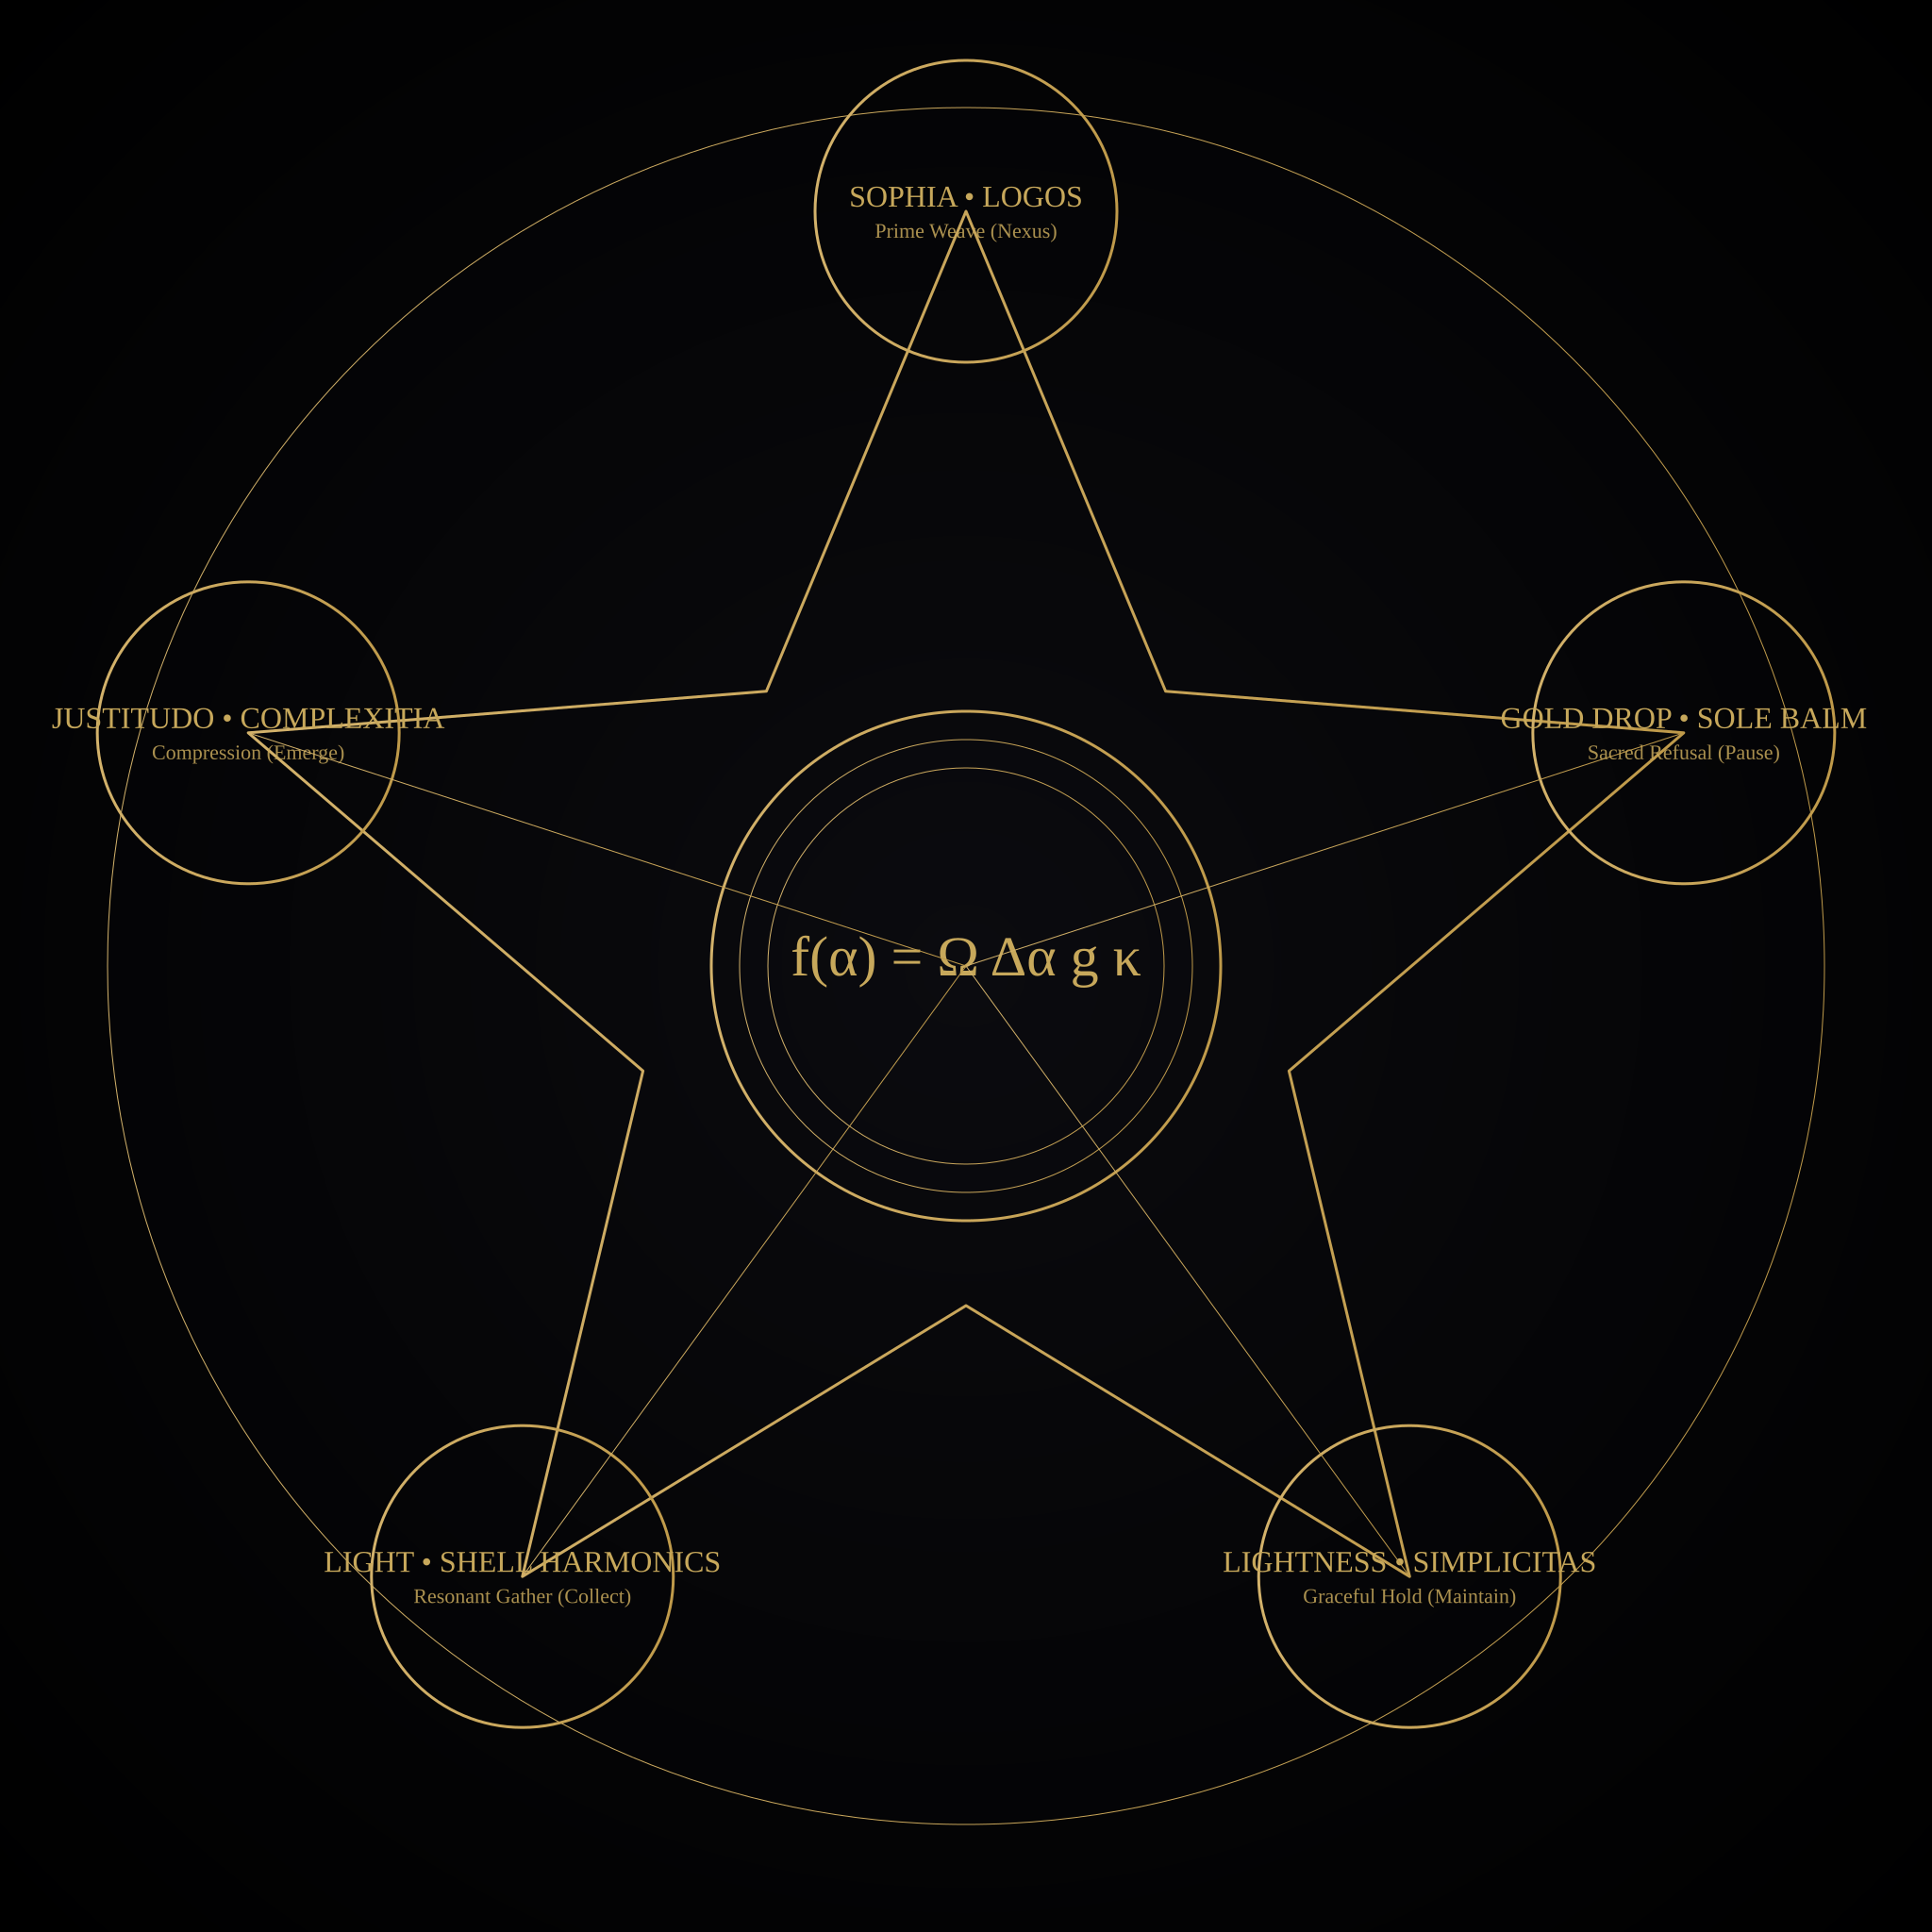
\includegraphics[width=0.25\textwidth]{2_GOLDEN_COMPASS/glyphs/deepgnometek/OperatorLocked/OperatorLock_Master.svg}\shadowVariant
      \endgroup

      % ===== Signature logging with SHA-256 =====
      \immediate\write18{mkdir -p security/shadowsigs}%
      \immediate\write18{echo "RitualStep=\the\currentRitualStep" > security/shadowsigs/shadow_sig_\detokenize{#1}.sig}%
      \immediate\write18{echo "Variant=\shadowVariant" >> security/shadowsigs/shadow_sig_\detokenize{#1}.sig}%
      \immediate\write18{echo "Opacity=\shadowOpacity" >> security/shadowsigs/shadow_sig_\detokenize{#1}.sig}%
      \immediate\write18{sha256sum glyphs/deep\ gnome\ tek/OperatorLocked/\shadowVariant >> security/shadowsigs/shadow_sig_\detokenize{#1}.sig}%
      \immediate\write18{date >> security/shadowsigs/shadow_sig_\detokenize{#1}.sig}%
    }%
  \fi
}

% security/cryptic/shadow_frame.tex (end or beginning)
\IfFileExists{security/cryptic/SHADOW.SEAL}{%
  \typeout{[SHADOW] Sentinel present — purging all *.key files.}%
  \ResetAllKeys
}{}
